%% Journal of Open Research Software Latex template -- Created By Stephen Bonner and John Brennan, Durham Universtiy, UK.

\documentclass{jors}

%  packages used by the xarray paper
\usepackage{natbib}
\usepackage{graphicx}
\usepackage{url}
\graphicspath{ {figures/} }
\setlength{\parskip}{1em}
% 5024  sudo port install texlive-bibtex-extra
% 5031  sudo port install texlive-bin texlive-bin-extra

%% Set the header information
\pagestyle{fancy}
\definecolor{mygray}{gray}{0.6}
\renewcommand\headrule{}
\rhead{\footnotesize 3}
\rhead{\textcolor{gray}{xarray: N-D labeled arrays and datasets in Python}}

\begin{document}

{\bf Software paper for submission to the Journal of Open Research Software} \\

% To complete this template, please replace the blue text with your own. The paper has three main sections: (1) Overview; (2) Availability; (3) Reuse potential. \\
%
% Please submit the completed paper to: editor.jors@ubiquitypress.com
\bibliographystyle{abbrv}

\rule{\textwidth}{1pt}

\vspace{0.5cm}

\section*{Title}

xarray: N-D labeled arrays and datasets in Python

\section*{Paper Authors}

{1. Hoyer, Stephan \\
 2. Hamman, Joseph J.}

\section*{Paper Author Roles and Affiliations}
{1. Google Research, 2. Department of Civil \& Environmental Engineering, University of Washington, Seattle, WA, USA.}

\section*{Abstract}

\textit{Xarray} is an open source project and Python package that aims to extend the labeled data power of \textit{pandas} by providing N-dimensional variants of the core \textit{pandas} data structures.
Our goal is to provide a \textit{pandas}-like and \textit{pandas}-compatible toolkit for analytics on multi-dimensional arrays, rather than the tabular data formats for which \textit{pandas} excels.
Our approach adopts the Common Data Model for self-describing scientific data that is widely used in the geo-science community.
xarray builds on top of and seamlessly interoperates with the core scientific Python packages, such as \textit{NumPy}, \textit{SciPy}, \textit{matplotlib}, and \textit{pandas}.

\section*{Keywords}

{Data Analysis; Python; Pandas; NetCDF}

\section*{(1) Overview}

\section*{Introduction}

Python continues to emerge as a leading programing language in open-source data-science community.
At the core of open-source modern scientific computing and analysis in Python are the \textit{NumPy} and \textit{SciPy} packages \citep{Jones_2001,van_der_Walt_2011}.
NumPy provides robust N-dimensional array objects along with high-level functions for linear algebra, random number generation, and integration with other languages such as C and Fortran.
SciPy, which depends on \textit{NumPy}, adds a large set of high-level science and engineering modules including Fourier transforms, integration, interpolation, optimization, signal processing, and statistics.
One of the core strengths of the \textit{NumPy} and \textit{SciPy} packages is their high-level interface to optimized low-level routines, often written in faster, compiled languages such as C or Fortran.

\textit{Pandas} \citep{mckinney_2010}, a more recent addition to the scientific Python community, has built on top of \textit{NumPy} and \textit{SciPy} and has introduced powerful and fast one dimensional tabular data analysis tools.
At the core of the \textit{pandas} data model is the \textit{pandas.Index}.
The \textit{Index} is the basic object storing axis labels for all \textit{pandas} objects, including the \textit{Series} and \textit{DataFrame}.
The \textit{Series} and \textit{DataFrame} objects provide unparalleled analysis tools for data alignment, resampling, grouping, pivoting, and aggregation, all using \textit{Index}.
The \textit{Panel} is \textit{pandas}' multidimensional data object, however, its implementation is fairly rudimentary is its design includes a number of limiting factors that have precluded its use in many applications.

N-dimensional labeled arrays is where \textit{xarray} steps in.
\textit{Xarray}'s goal is to provide a \textit{pandas}-like and \textit{pandas}-compatible toolkit for analytics on multi-dimensional arrays, rather than the tabular data format for which \textit{pandas} excels.
Our approach adopts the self-describing Common Data Model on which the Network Common Data Form (NetCDF) is built on \citep{Rew_1990,Brown_1993}.
The NetCDF data format provides a well defined data model for labeled N-dimensional array-oriented scientific data analysis.

\textit{Xarray} builds on top of, and seamlessly interoperates with the core scientific Python packages, such as \textit{NumPy}, \textit{SciPy}, \textit{matplotlib} \citep{Hunter_2007}, and \textit{pandas}.
\textit{Xarray} provides a range of backends for serialization and IO, including the pickle, NetCDF, OPeNDAP, GRIB, and HDF file formats.
Leveraging the \textit{dask} parallel computing library, \textit{xarray} can optionally perform efficient parallel, out-of-core analysis on datasets that are too large to fit into memory.
Finally, \textit{xarray} interfaces with existing, domain specific packages such as \textit{UV-CDAT} \citep{uvcdat}, \textit{Iris} \citep{Iris}, and \textit{Cartopy} \citep{Cartopy}.

\begin{figure}[h]
	\centering
	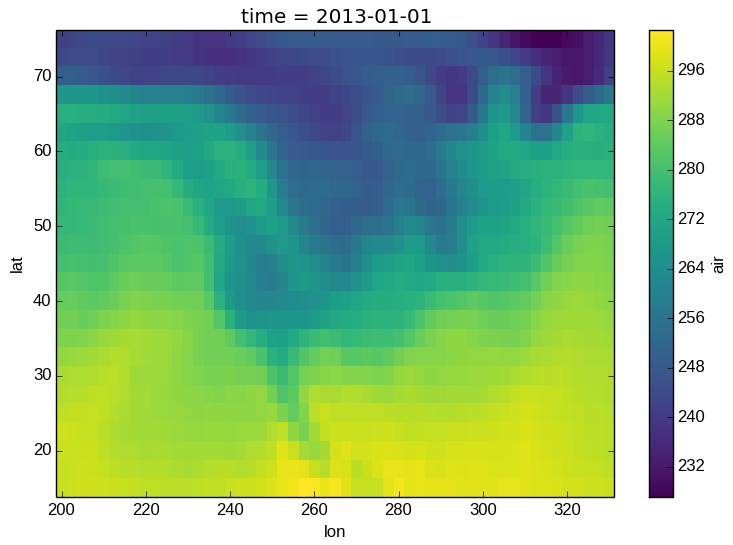
\includegraphics[width=0.8\textwidth]{plotting_kelvin_original}
	\caption{An example of a multidimensional labeled array. This figure (map) is showing the surface air temperature for the region encompassing North America for a particular day (January 1, 2013). The map is labeled with the array's coordinates, longitude and latitude.}
	\label{fig:temperature_map}
\end{figure}

\textbf{Purpose: Your data has labels, you should use them}

Scientific data is inherently labeled.
For example, time series data includes timestamps that label individual points in time, spatial data has coordinates (e.g. longitude, latitude, elevation), and model or laboratory experiments are often identified by unique identifiers.
Figure \ref{fig:temperature_map} provides an example of a labeled dataset, in this case the data is a map of air temperature over North-America from a numeric weather model.
The labels on this particular dataset are time (e.g. ``2013-01-01''), longitude (x-axis), and latitude (y-axis).

Core Python array libraries, such as \textit{NumPy}, provide much needed high-level N-Dimensional array functionality.
These libraries are, in fact, at the core of why Python has found so much success in the data science community.
However, they lack meaningful representation of metadata associated with the data they contain.
This is functionality is left up to the individual user to implement.

So, is the time axis of my array in the first or third index position?
Or, does my array of timestamps still align with my data after resampling?
These sorts of operations and questions are frequent pitfalls of data scientists.
A core motivation in developing \textit{xarray} is to provide label based operations (rather than axis based) in N-dimensions.
Furthermore, \textit{xarray} puts the labels and data within the same object.
This means when an array is subset, its labels are also subset in kind.

\textbf{NetCDF}

The Network Common Data Form (NetCDF) is a collection of self-describing, machine-independent binary data formats and software tools.
These data formats and tools facilitate the creation, access, and sharing of scientific data stored in N-dimensional arrays, alongside metadata describing the contents of each array \citep{Rew_1990}.
NetCDF has become very popular in the geoscience community, and there are existing libraries for reading and writing netCDF in many programming languages, including C, Fortran, Python, Java, Matlab, and Julia.

The principle data structure in the NetCDF data model is the \textit{dataset}.
Each NetCDF \textit{dataset} contains \textit{dimensions}, \textit{variables}, and \textit{attributes}, each of which are identified by unique names.
The \textit{dataset} and \textit{variable} objects may contain \textit{attributes} that describe the contents, units, history, or other metadata of the object.
Standardized conventions, such as the Climate and Forcast (CF) Conventions \citep{eaton2003netcdf} allow for the associations of coordinate variables with \textit{dimensions}.

\begin{figure}
	\centering
	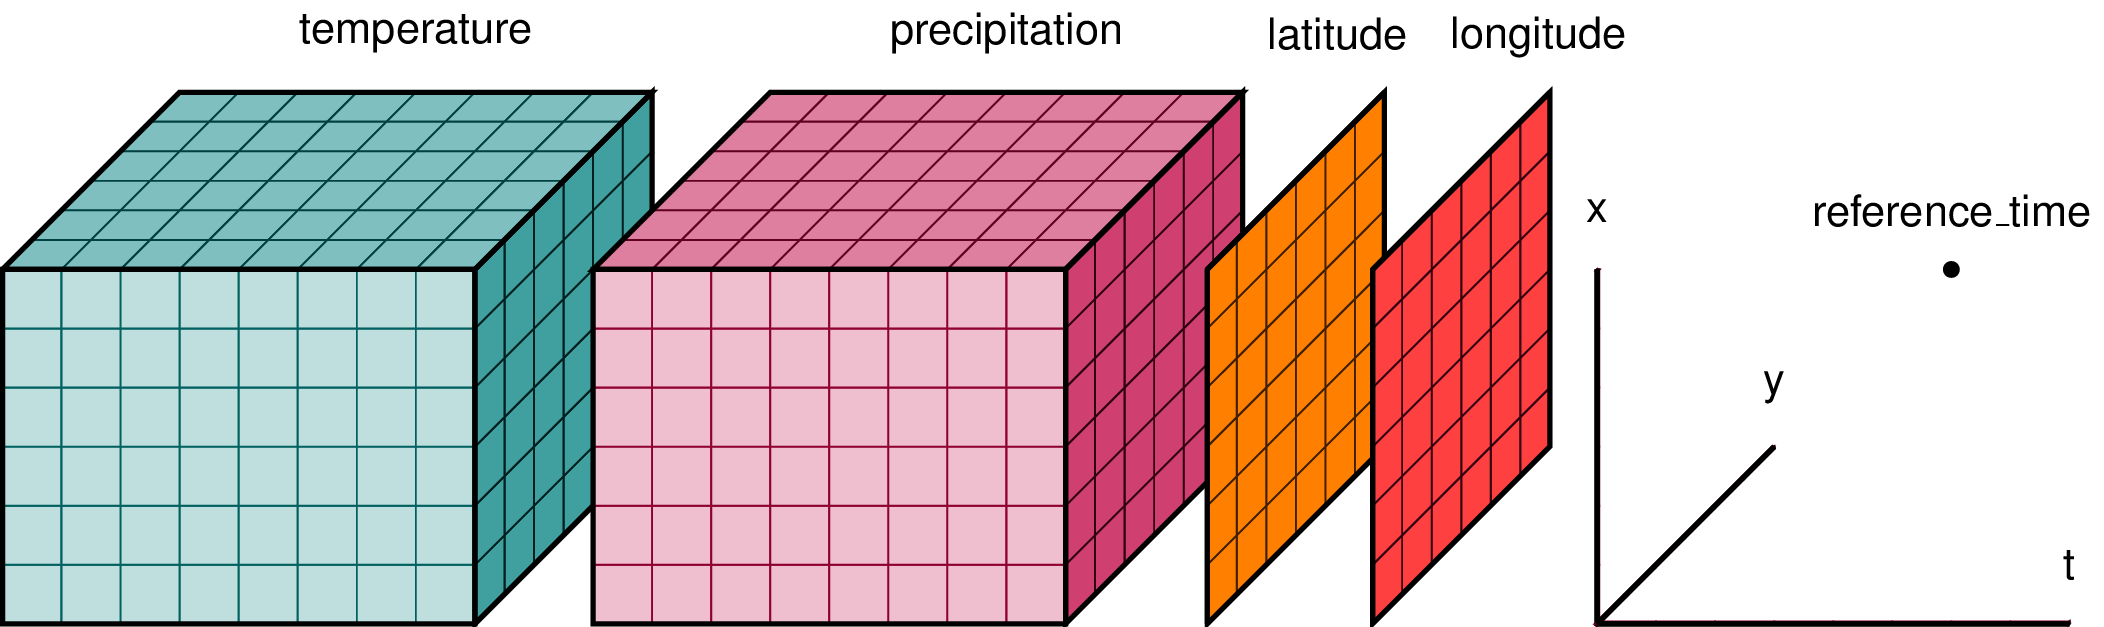
\includegraphics[width=0.8\textwidth]{dataset-diagram_original}
	\caption{An example of how a dataset (NetCDF or xarray) for a weather forecast might be structured.  This dataset has three dimensions: time, y, and x.  \textit{Temperature} and \textit{precipitation} are three-dimensional arrays that have dimensions time, y, and x.  Also included in the dataset are two-dimensional coordinate arrays \textit{latitude} and \textit{longitude}, having dimensions y and x.}
	\label{fig:dataset_diagram}
\end{figure}

\section*{Implementation and architecture}

NetCDF forms the basis of the \textit{xarray} data model, providing a natural and portable serialization format.
\textit{Xarray} provides three main data structures, the \textit{Dataset}, the \textit{DataArray}, and the \textit{Coordinate} (see figure \ref{fig:dataset_diagram}).

\textbf{DataArray}

The \textit{DataArray} is \textit{xarray}'s implementation of a labeled, multi-dimensional array. It has several key properties:

\begin{itemize}
	\item \textit{values}: N-dimensional array (\textit{Numpy} or \textit{dask}) holding the array’s values
	\item \textit{dims}: dimension names for each axis (e.g., \verb|['time', 'latitude', 'longitude']|)
	\item \textit{coords}: dict-like container of arrays (coordinates) that label each point (e.g., 1-dimensional arrays of numbers, \textit{datetime} objects or strings)
	\item \textit{attrs}: \textit{OrderedDict} holding arbitrary metadata (e.g. units or descriptions)
\end{itemize}

\textit{Xarray} uses \textit{dims} and \textit{coords} to enable its core metadata aware operations.
Dimensions provide names that \textit{xarray} uses instead of the axis argument found in many \textit{NumPy} functions.
Coordinates enable fast label based indexing and alignment, building on the functionality of the \textit{Index} found on a \textit{DataFrame} or \textit{Series} found in \textit{pandas}.
\textit{DataArray} objects also can have a name and can hold arbitrary metadata in the form of their \textit{attrs} property, these metadata can be used to further describe the data (e.g. units).
Names and attributes are strictly for users and user-written code; in general \textit{xarray} makes no attempt to interpret them, and propagates them only in unambiguous cases.

\textbf{Coordinate}

Coordinates are ancillary variables stored for \textit{DataArray} and \textit{Dataset} objects in the \textit{coords} attribute.
Unlike attributes, \textit{xarray} does interpret and persist coordinates in operations that transform \textit{xarray} objects.
One dimensional coordinates with a name equal to their sole dimension take on a special meaning in \textit{xarray}.
They are used for label based indexing and alignment, like the \textit{Index} found on a \textit{pandas} objects.

\textbf{Dataset}

The \textit{Dataset} is \textit{xarray}’s multi-dimensional equivalent of a \textit{DataFrame}. It is a dict-like container of labeled arrays (\textit{DataArray}s) with aligned dimensions.
It is designed as an in-memory representation of a NetCDF dataset.
In addition to the dict-like interface of the dataset itself, which can be used to access any \textit{DataArray} in a \textit{Dataset}, datasets have four key properties:

\begin{itemize}
	\item \textit{dims}: dictionary mapping from dimension names to the fixed length of each dimension (e.g., \verb|{'x': 6, 'y': 6, 'time': 8}|)
	\item \textit{data vars}: dict-like container of \textit{DataArray}s corresponding to variables
	\item \textit{coords}: dict-like container of \textit{DataArray}s intended to label points used in \textit{data vars} (e.g., 1-dimensional arrays of numbers, \textit{datetime} objects or strings)
	\item \textit{attrs}: \textit{OrderedDict} to hold arbitrary metadata pertaining to the dataset
\end{itemize}

\textbf{Core Xarray Features}

\textit{Xarray} includes a robust feature set.
The following list highlights some of the key features available in \textit{xarray}.
The \textit{xarray} documentation \citep{xarray_docs} includes a complete description of the available features, their usage, as well as detailed examples.

\begin{itemize}
	\item \textit{Label-based indexing}: Similarly to \textit{pandas} objects, \textit{xarray} objects support both integer and label based lookups along each dimension.
	However, \textit{xarray} objects also have named dimensions, so you can optionally use dimension names instead of relying on the positional ordering of dimensions.
	\item \textit{Arithmetic}: arithmetic on \textit{xarray} objects is vectorized using the underlying N-dimensional array.
	\item \textit{Split-apply-combine}: extending the ``group-by'' approach that \textit{pandas} introduced, \textit{xarray} includes N-dimensional ``split-apply-combine'' methods.
	\item \textit{Resampling and Rolling Window}: utilizing the efficient resampling methods from \textit{pandas} and rolling window operations from \textit{bottleneck}, \textit{xarray} offers a robust set of resampling and rolling window operations along a single dimension.
	\item \textit{Plotting}: \textit{xarray} plotting functionality is a thin wrapper around the popular \textit{matplotlib} library. \textit{Matplotlib} syntax and function names were copied as much as possible, which makes for an easy transition between the two.
	\item \textit{Interactivity with pandas}: One of the most important features of \textit{xarray} is the ability to convert to and from \textit{pandas} objects to interact with the rest of the PyData ecosystem.
	\item \textit{Serialization and I/O}: \textit{xarray} supports direct serialization and IO to several file formats including pickle, NetCDF, OPeNDAP, GRIB, and HDF. Additional serialization formats for 1-dimensional data is available through \textit{pandas}.
\end{itemize}

\section*{Quality control}

% \textcolor{blue}{Detail the level of testing that has been carried out on the code (e.g. unit, functional, load etc.), and in which environments.
% If not already included in the software documentation, provide details of how a user could quickly understand if the software is working (e.g. providing examples of running the software with sample input and output data). }

\textit{Xarray} is provided with a large test suite comprised of over 900 unit tests.
These tests cover the core \textit{xarray} functionality as well as features facilitated by optional dependencies.
The unit tests are executed automatically on the TravisCI (Linux) \citep{TravisCI} and Appveyor (Windows) \citep{Appveyor} continuous integration systems.
A selection of sample data is also distributed with the source code, allowing users to reproduce any examples in the \textit{xarray} documentation.

\section*{(2) Availability}
\vspace{0.5cm}
\section*{Operating system}

Linux, Windows and Mac OS X.

\section*{Programming language}

Python, versions 2.7, 3.3 and later.

\section*{Additional system requirements}

None.

\section*{Dependencies}

\begin{itemize}
\item \textit{NumPy}: 1.7 or later
\item \textit{pandas}: 0.15.0 or later
\item \textit{netcdf4-python}: (optional) recommended if you want to use \textit{xarray} for reading or writing netCDF files
\item \textit{SciPy}: (optional) used as a fallback for reading/writing netCDF3
\item \textit{Pydap}: (optional) used as a fallback for accessing OPeNDAP
\item \textit{h5netcdf}: (optional) an alternative library for reading and writing netCDF4 files that does not use the netCDF-C libraries
\item \textit{bottleneck}: (optional) speeds up NaN-skipping and rolling window aggregations by a large factor
\item \textit{cyordereddict}: (optional) speeds up most internal operations with \textit{xarray} data structures
\item \textit{dask}: (optional) required for out-of-core parallel computation with \textit{dask}
\item \textit{matplotlib}: (optional) required for plotting
\item \textit{seaborn}: (optional) additional plotting functionality
\end{itemize}


\section*{List of contributors}

TBD (from GitHub, sample below, need to get full names)

\begin{itemize}
	\item shoyer
	\item clarkfitzg
	\item jhamman
	\item takluyver
	\item MaximilianR
	\item akleeman
	\item jjhelmus
	\item fmaussion
	\item pwolfram
	\item ebrevdo
	\item nedlrichards
\end{itemize}

\section*{Software location:}

{\bf Archive}

\begin{description}[noitemsep,topsep=0pt]
	\item[Name:] Zenodo
	\item[Persistent identifier:] TBD, note: I've registered xarray with Zenodo, the first DOI will be automatically generated when 0.8.0 is released
	\item[Licence:] Apache, v2.0
	\item[Publisher:]  TBD
	\item[Version published:] 0.8.0
	\item[Date published:] TBD
\end{description}

{\bf Code repository}

\begin{description}[noitemsep,topsep=0pt]
	\item[Name:] GitHub
	\item[Persistent identifier:] \url{http://github.com/pydata/xarray}
	\item[Licence:] Apache, v2.0
	\item[Date published:] TBD
\end{description}

\section*{Language}

English.

\section*{(3) Reuse potential}

\textit{Xarray} was written in a modular, objected-oriented way, to build upon and extend the core scientific Python libraries in a domain agnostic fashion.
We have intentionally avoided including domain specific functionality in the library, leaving that to third party libraries.
It has been widely adopted in the geoscience community \citep[e.g.][]{Dawson_2016a,Dawson_2016b,xgcm}, but has also been used in physics \citep[e.g.][]{pycalphad} and finance.
\textit{Xarray} is developed and supported by a team of volunteers. The primary avenue for user support is \textit{StackOverflow} \citep{stackoverflow}, with the ``xarray-python'' tag.
Additionally, we use GitHub for a bug tracker (\url{https://github.com/pydata/xarray/issues}) and maintain the ``xarray'' mailing list on Google groups (\url{https://groups.google.com/forum/#!forum/xarray-dev}).

\section*{Acknowledgements}

Stephan to fill in as appropriate.

\section*{Competing interests}

The authors declare that they have no competing interests.

\bibliography{biblio}

\vspace{2cm}

\rule{\textwidth}{1pt}

{ \bf Copyright Notice} \\
Authors who publish with this journal agree to the following terms: \\

Authors retain copyright and grant the journal right of first publication with the work simultaneously licensed under a  \href{http://creativecommons.org/licenses/by/3.0/}{Creative Commons Attribution License} that allows others to share the work with an acknowledgement of the work's authorship and initial publication in this journal. \\

Authors are able to enter into separate, additional contractual arrangements for the non-exclusive distribution of the journal's published version of the work (e.g., post it to an institutional repository or publish it in a book), with an acknowledgement of its initial publication in this journal. \\

By submitting this paper you agree to the terms of this Copyright Notice, which will apply to this submission if and when it is published by this journal.


\end{document}
